\newpage
\section{Results}
\subsection{The Change in Aerosol Concentrations}
After applying the high-pressure blocking detection method to the data from Vavihill and Malmö for the entire period, a total of 213 high-pressure blocking events were identified between November 27, 1995 and September 22, 2024. For Vavihill 114 high-pressure blocking events of the original 213 were removed due to insufficient \PM data, as a filter requiring 85\% data coverage was applied. This left 99 relevant high-pressure blocking events. For Malmö 48 high-pressure blocking events were removed due to insufficient \PM data, again applying the 85\% data coverage filter. This resulted in 165 relevant high-pressure blocking events. An example plot showing periods of high-pressure blocking events can be seen in \autoref{fig:2001}. This figure provides insight into the categorization of high-pressure blocking events for the two different locations.  

\begin{figure}[H]
    \centering
    \begin{subfigure}[b]{0.49\textwidth}
        \centering
        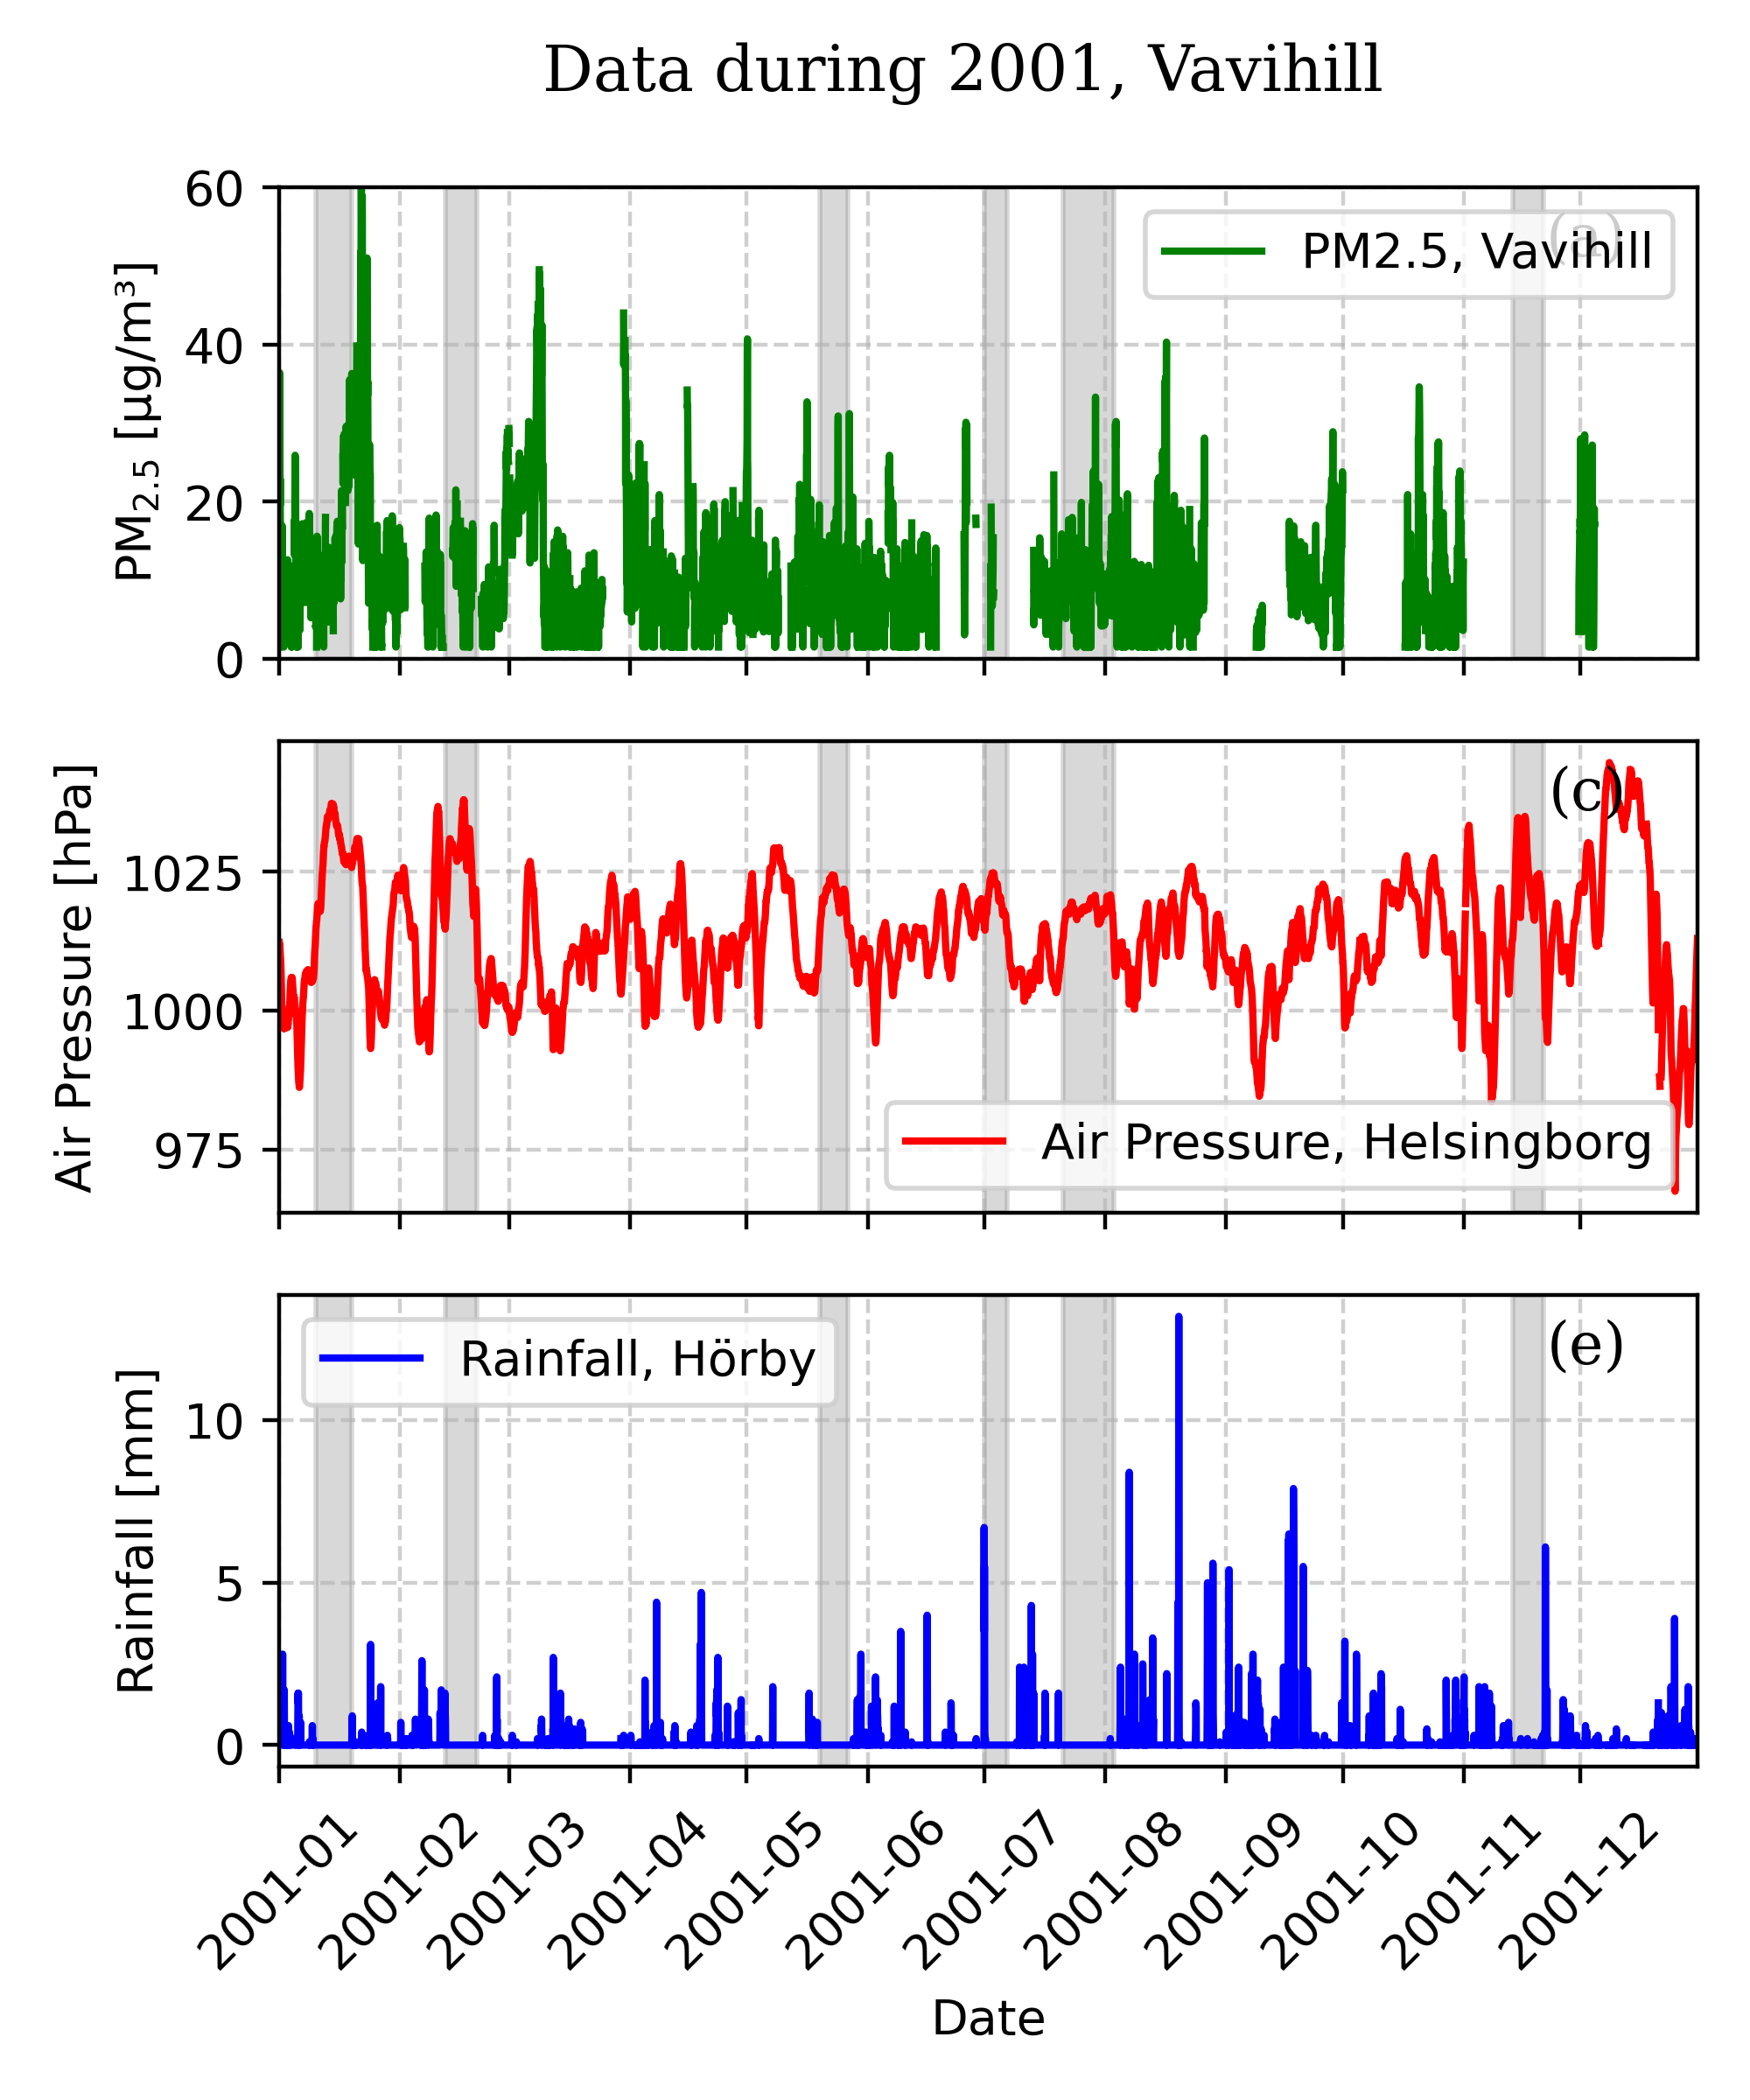
\includegraphics[width=\textwidth]{Figures/Vavihill_plot_20010101_20011231.png}
        \label{fig:2001Vavihill}
    \end{subfigure}
    \hfill
    \begin{subfigure}[b]{0.49\textwidth}
        \centering
        \includegraphics[width=\textwidth]{Figures/Malmö_plot_20010101_20011231.png}
        \label{fig:2001Malmö}
    \end{subfigure}
    \caption{Example plots displaying the air pressure, \PM concentrations, and rainfall during the year 2001. The periods which were indicated as periods of high-pressure blocking events are shaded in gray. This displays a normal yearly distribution of high-pressure blocking events using the described method.}
    \label{fig:2001}
\end{figure}

The average change in \PM concentrations during periods of high-pressure blocking can be seen in \autoref{fig:Meanplot_Comparison}. The data is compared with the \PM mean taken from periods without high-pressure blocking events. An increase in \PM concentrations can be seen in Malmö from \SI{10}{\micro\gram\per\meter\cubed} to a maximum of \SI{21}{\micro\gram\per\meter\cubed} at day thirteen, and an increase from \SI{7}{\micro\gram\per\meter\cubed} to a maximum of \SI{18}{\micro\gram\per\meter\cubed} at day twelve can be seen in Vavihill. The increase is supported by the large $\tau$-value of $\tau=0.78$ in Malmö, and slight lower $\tau=0.70$ in Vavihill. The Sen's slope values also indicate a stronger increase in Malmö \SI{3.0e-02}{\micro\gram\per\meter\cubed\per\day} compared to \SI{2.1e-02}{\micro\gram\per\meter\cubed\per\day} in Vavihill. After the first five days, the number of high-pressure blocking events decreases, which is reflected in the increase in standard deviation. 


\begin{figure}[H]
    \centering
    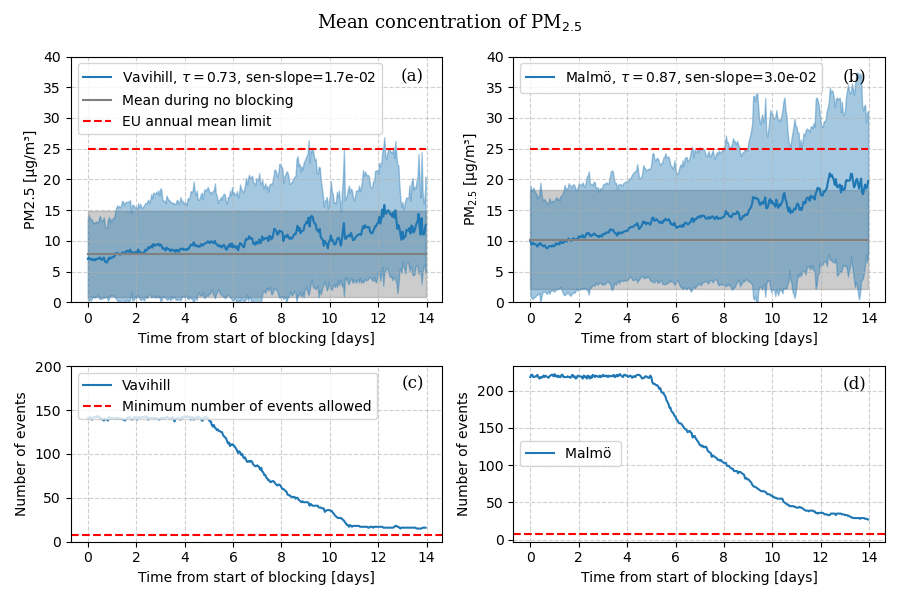
\includegraphics[width=\textwidth]{Figures/Meanplot.png}
    \caption{Mean \PM concentrations in Vavihill (a) and Malmö (b) during high-pressure blocking events (blue line). The grey line shows the mean \PM during non-high pressure blocking events. The shaded region indicates the standard deviation of the data. The number of high-pressure blocking events used in the analysis can be seen in (c) and (d), where the minimum number of events allowed was shown by the red line. }
    \label{fig:Meanplot_Comparison}
\end{figure}


The average change in \PM concentrations after periods of high-pressure blocking can be seen in \autoref{fig:Meanplot_after}. Observing this plot one can observe that after the end of a high-pressure blocking event the \PM levels return to normal during the first day after the end of the event. This is an interesting result which highlights that the increase observed in \autoref{fig:Meanplot_Comparison}, is indeed due to the presence of a high-pressure blocking event. This behaviour should be expected since high-pressure blocking event often end in rainfall, or change of wind direction which would contribute to a fast decrease in aerosols concentrations. 

\begin{figure}[H]
    \centering
    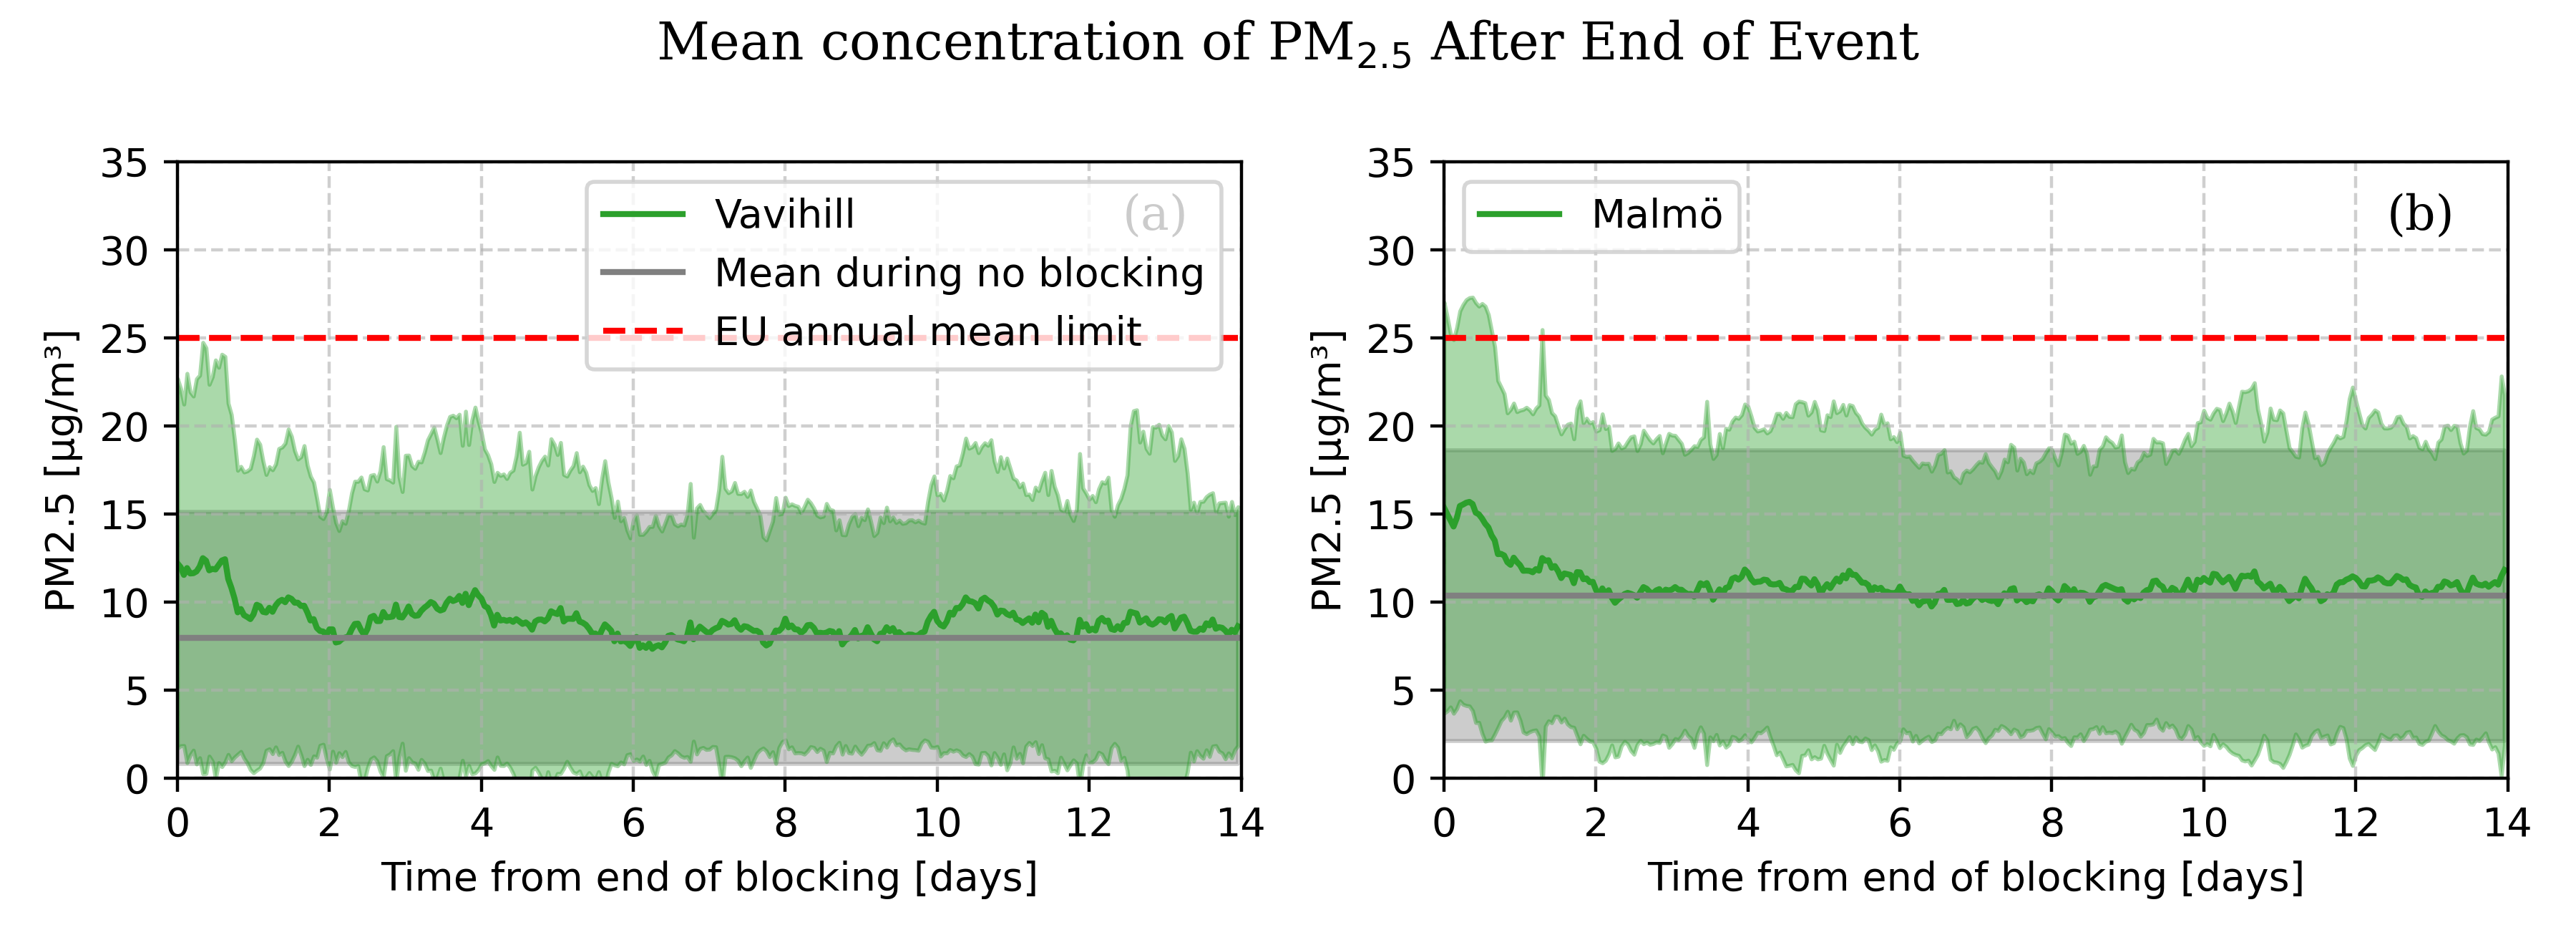
\includegraphics[width=\textwidth]{Figures/Meanplot_after.png}
    \caption{Mean \PM concentrations in Vavihill (a) and Malmö (b) after the end of high-pressure blocking events (green line). The grey line shows the mean \PM during non-high pressure blocking events. The shaded region indicates the standard deviation of the data.  }
    \label{fig:Meanplot_after}
\end{figure}


\subsubsection{The Change in Aerosol Concentrations Depending on Wind Direction}

The change in \PM concentrations in Vavihill and Malmö during high-pressure blocking events for different wind directions can be seen in \autoref{fig:Meanplot_wind}. In the case of Vavihill, 7.1\% of the winds came from the northeast (310° to 70°), 27.3\% from the southeast (70° to 190°), 23.2\% from the west (190° to 310°) and 42.4\% from no specific direction. In the case of Malmö, 7.9\% of the winds came from the northeast (310° to 70°), 24.8\% from the southeast (70° to 190°), 18.2\% from the west (190° to 310°) and 49.1\% from no specific direction. Very little data is observed from the northeast because this is a uncommon wind direction during high-pressure blocking events as seen in \autoref{fig:map}. A large proportion of the data was categorized as "no specific", since the movement of the high-pressure blocking event usually results in changing wind directions. 


One can observe similarities between the aerosol concentrations depending on wind directions for Vavihill and Malmö, although a larger increase can be observed in Malmö. When only considering the northeast direction, no strong increase or high levels of \PM were detected, as supported by the $\tau$-values being under 0.5 for Malmö, and no statistically significant amount of data being found at Vavihill (\autoref{fig:Meanplot_wind}a-b). In Vavihill the southeastern direction yielded $\tau=0.41$, however there is a clear increase until day nine, where the levels suddenly drop (\autoref{fig:Meanplot_wind}c). The $\tau$-value for the first nine days is $\tau=0.68$, showing a clear increase. The southeastern direction for Malmö yielded a high $\tau$-value of $\tau=0.64$ and mean concentration exceeding the EU annual mean limit with a maximum concentration of \SI{26}{\micro\gram\per\meter\cubed}(\autoref{fig:Meanplot_wind}d). For the western wind direction, an increase in \PM can be seen in Vavihill as supported by $\tau=0.57$ (\autoref{fig:Meanplot_wind}e). The western wind direction for Malmö showed an increase until day eight, where it suddenly drops. Although elevated levels can be seen on day eight, one must note that the spread of the values is large (\autoref{fig:Meanplot_wind}f). The non specific direction in \autoref{fig:Meanplot_wind}g-h showed increases similar to the increase in \autoref{fig:Meanplot_Comparison}. This category shows that when the wind direction is changing a monotonic increase is observed, supported by $\tau=0.70$ in Vavihill and $\tau=0.79$ in Malmö. 

\begin{figure}[H]
    \centering
    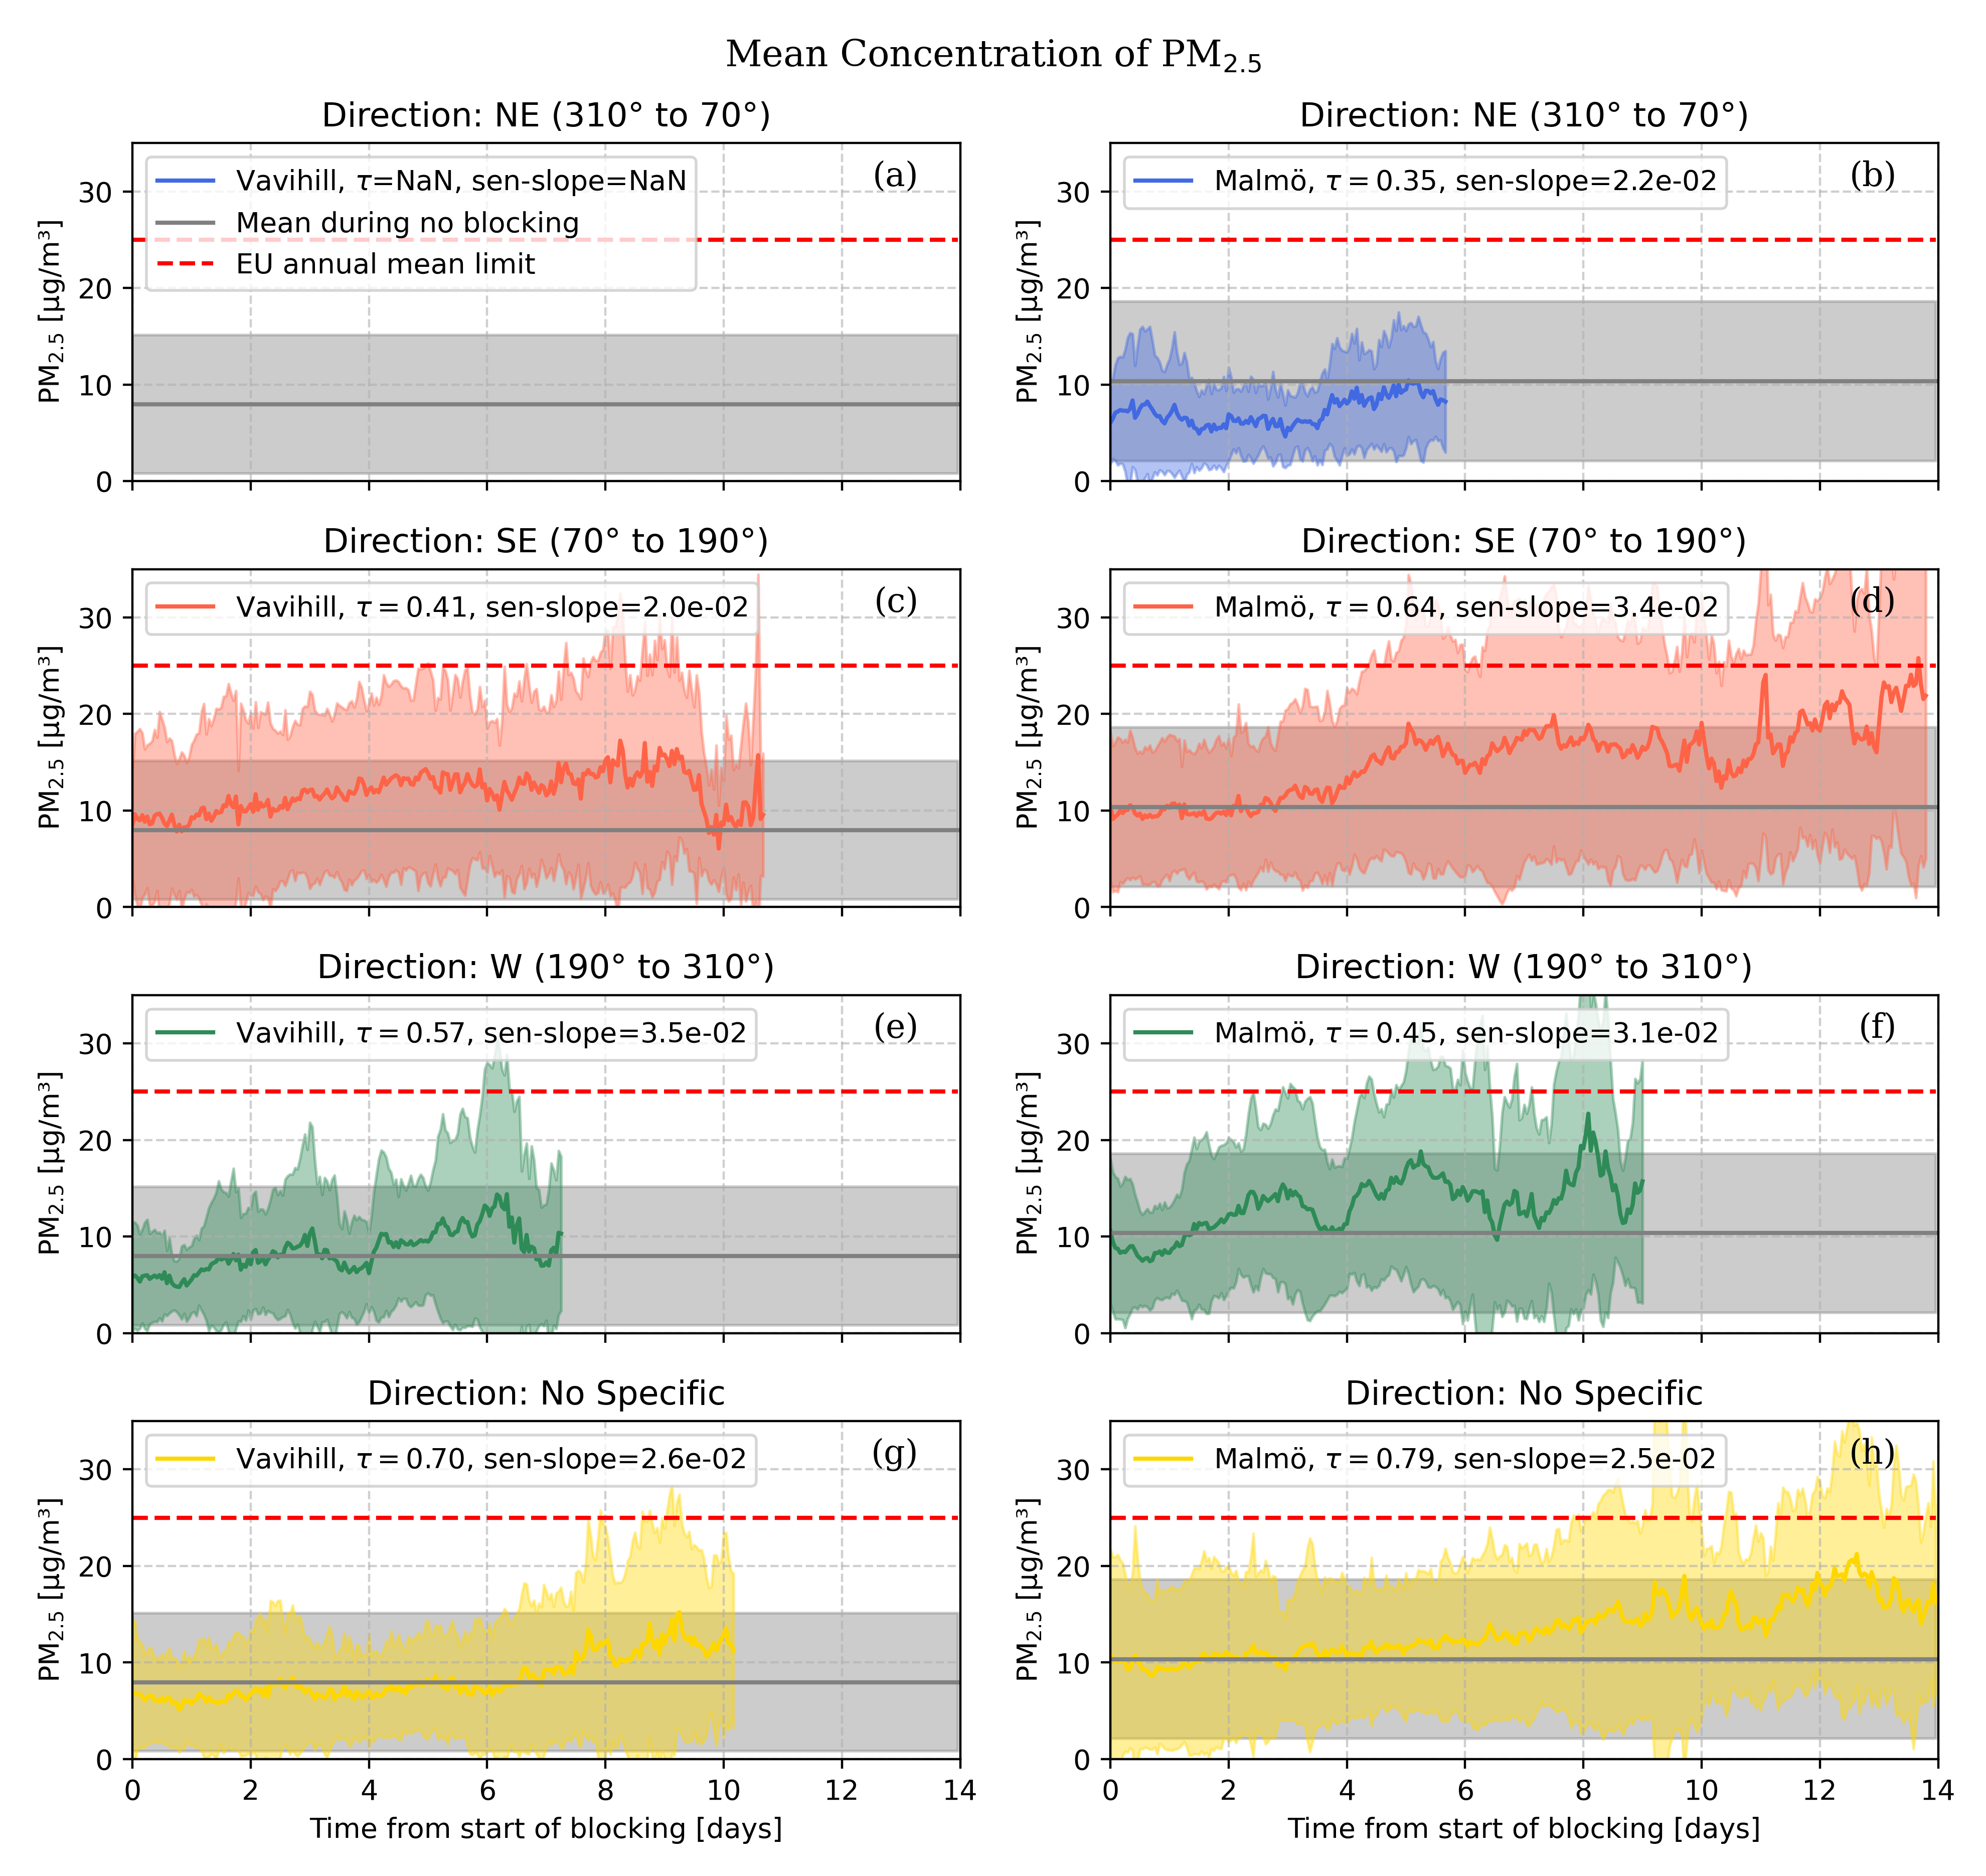
\includegraphics[width=\textwidth]{Figures/Meanplot_dir.png}
    \caption{\PM concentrations evolution in Vavihill and Malmö for different wind directions during high-pressure blocking events. This is shown by the blue line, the mean during no high-pressure blocking event can be seen by the grey line and the EU annual mean limit is displayed by the red line. The shaded regions indicates the standard deviation of the data. Figure (a) is empty due to insufficient amount of data for the northeastern category in Vavihill. }
    \label{fig:Meanplot_wind}
\end{figure}



\subsubsection{The Change in Aerosol Concentrations Depending on Season}
The seasonal change in concentrations of \PM during high-pressure blocking events can be seen in \autoref{fig:Meanplot_seasonal}. 19.8\% of the events occurred during the winter, 32.8\% during the spring, 19.8\% during the summer and 27.6\% during the autumn. From \autoref{fig:Meanplot_seasonal} e-f, it is clear that the concentration during the summer for both Vavihill and Malmö does not show an increase nor high levels of \PM. A slight increase can be seen for the spring in both locations, with Vavihill going from \SI{9}{\micro\gram\per\meter\cubed} to a maximum of \SI{12}{\micro\gram\per\meter\cubed}, and Malmö from \SI{11}{\micro\gram\per\meter\cubed} to a maximum of \SI{16}{\micro\gram\per\meter\cubed} (\autoref{fig:Meanplot_seasonal}c-d). A larger increase can be seen during the autumn (\autoref{fig:Meanplot_seasonal}g-h), where high levels of \PM can be observed towards the end of the period, with Vavihill going from \SI{10}{\micro\gram\per\meter\cubed} to a maximum of \SI{16}{\micro\gram\per\meter\cubed}, and Malmö from \SI{11}{\micro\gram\per\meter\cubed} to a maximum of \SI{26}{\micro\gram\per\meter\cubed}. During the winter, an increase in the \PM concentrations were observed, with Malmö showing a much stronger increase which is supported by $\tau=0.70$ and the Sen's slope being \SI{6.9e-02}{\micro\gram\per\meter\cubed\per\day} (\autoref{fig:Meanplot_seasonal}a-b). 

\begin{figure}[H]
    \centering
    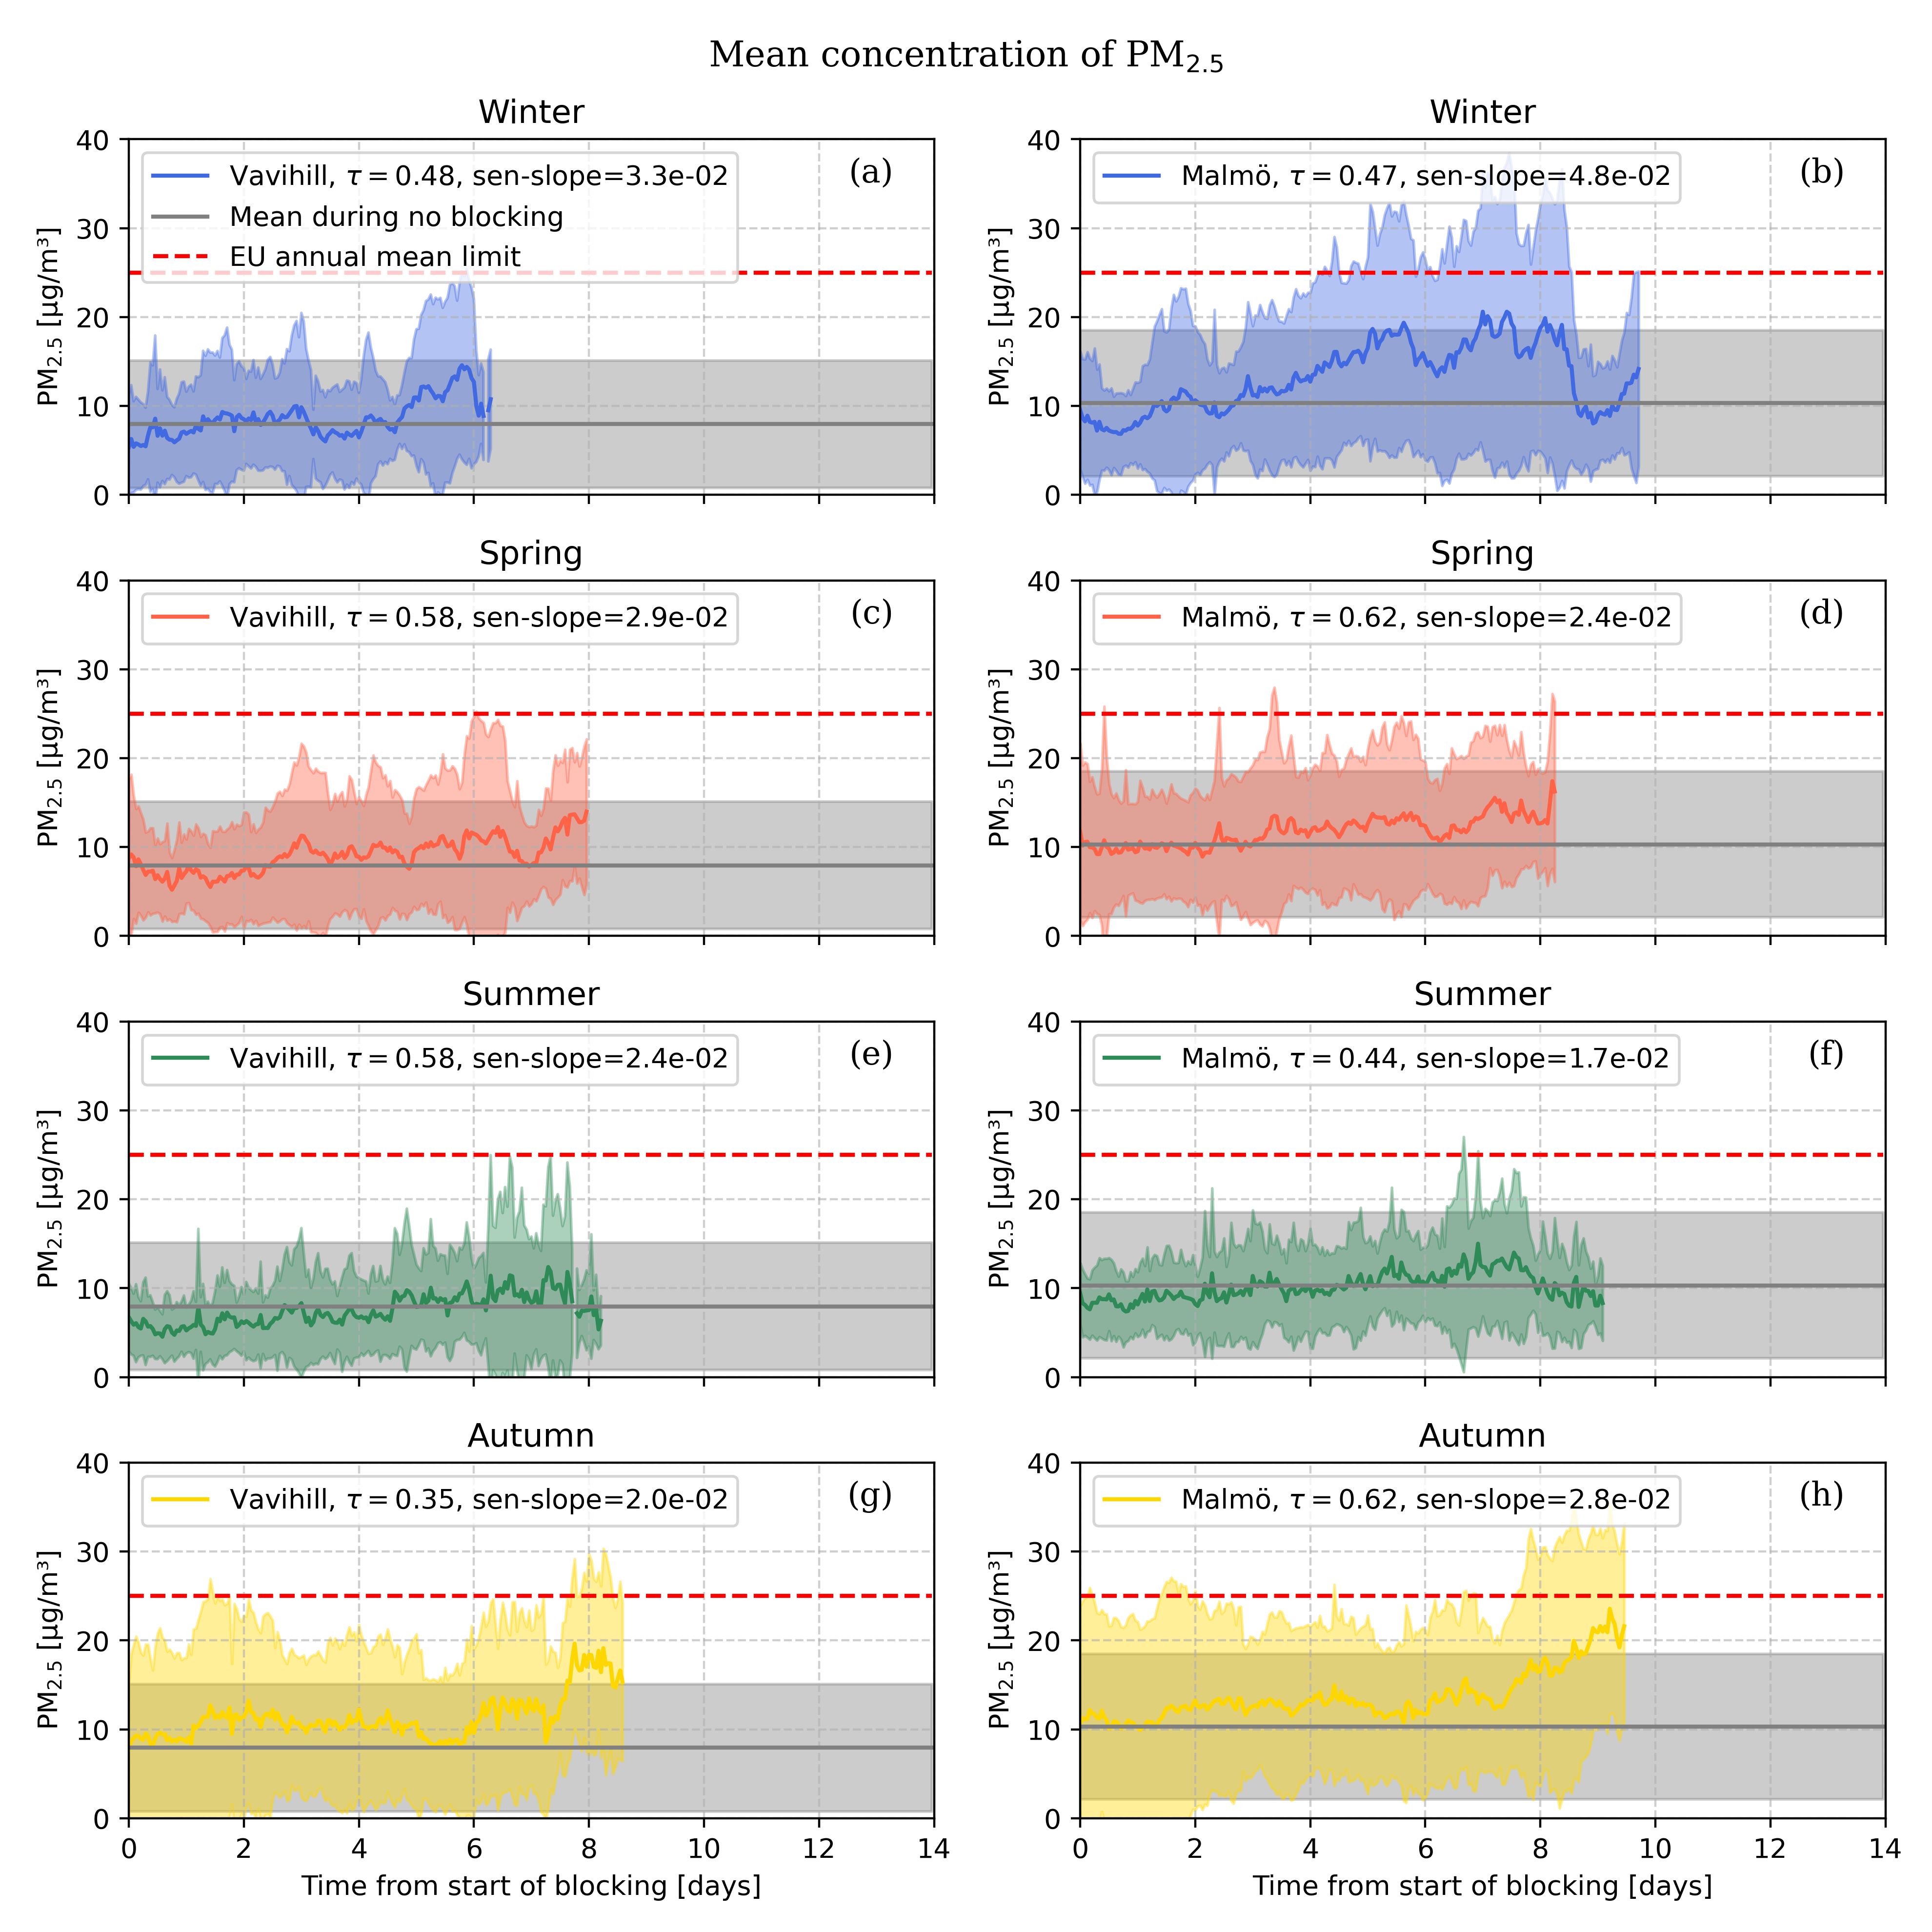
\includegraphics[width=\textwidth]{Figures/Meanplot_seasonal.png}
    \caption{\PM concentrations in Vavihill and Malmö during high-pressure blocking events for different seasons. This is shown by the blue line, the mean during no high-pressure blocking event can be seen by the grey line and the EU annual mean limit is displayed by the red line. The shaded regions indicates the standard deviation of the data.}
    \label{fig:Meanplot_seasonal}
\end{figure}
 

\subsubsection{The Change in Aerosol Concentrations Depending on Pressure Strength}
The increase in \PM concentrations depending on the strength of the high-pressure blocking event can be seen in \autoref{fig:Meanplot_pressure}. In the case of Vavihill, 22.2\% of the blocking events occurred with a mean pressure below 1020 hPa 45.5\% occurred between 1020 and 1025 hPa and 31.3\% occurred with a mean pressure over 1025hPa. In the case of Malmö, 17.0\% of the blocking events occurred with a mean pressure below 1020 hPa 48.5\% occurred between 1020 and 1025 hPa and 34.5\% occurred with a mean pressure over 1025hPa.


From the plots, one can observe similar behaviour for the two locations. For the weaker high-pressure blocking events no prolonged increase can be seen for Malmö, nor highly elevated levels of \PM in either location (\autoref{fig:Meanplot_pressure}a-b). In the case of medium strong high-pressure blocking events a stronger increase in Vavihill $\tau=0.62$ and weaker in Malmö $\tau=0.30$ can be seen. When observing both plots one can see a maximum around day nine, although the maximum in Malmö has a larger value spread (\autoref{fig:Meanplot_pressure}c-d). For the stronger high-pressure blocking events one can see a strong increase in the case of Malmö and in Vavihill, although the increase in Vavihill is slightly weaker. When viewing the plots \autoref{fig:Meanplot_pressure}e-f one observes that the levels of \PM in the case of Vavihill and Malmö exceed the normal range at day thirteen, where the mean reached the EU annual mean limit for Malmö. In Vavihill the values went from \SI{9}{\micro\gram\per\meter\cubed} to a maximum of \SI{21}{\micro\gram\per\meter\cubed}, and in Malmö they went from \SI{12}{\micro\gram\per\meter\cubed} to a maximum of \SI{28}{\micro\gram\per\meter\cubed}. 


\begin{figure}[H]
        \centering
        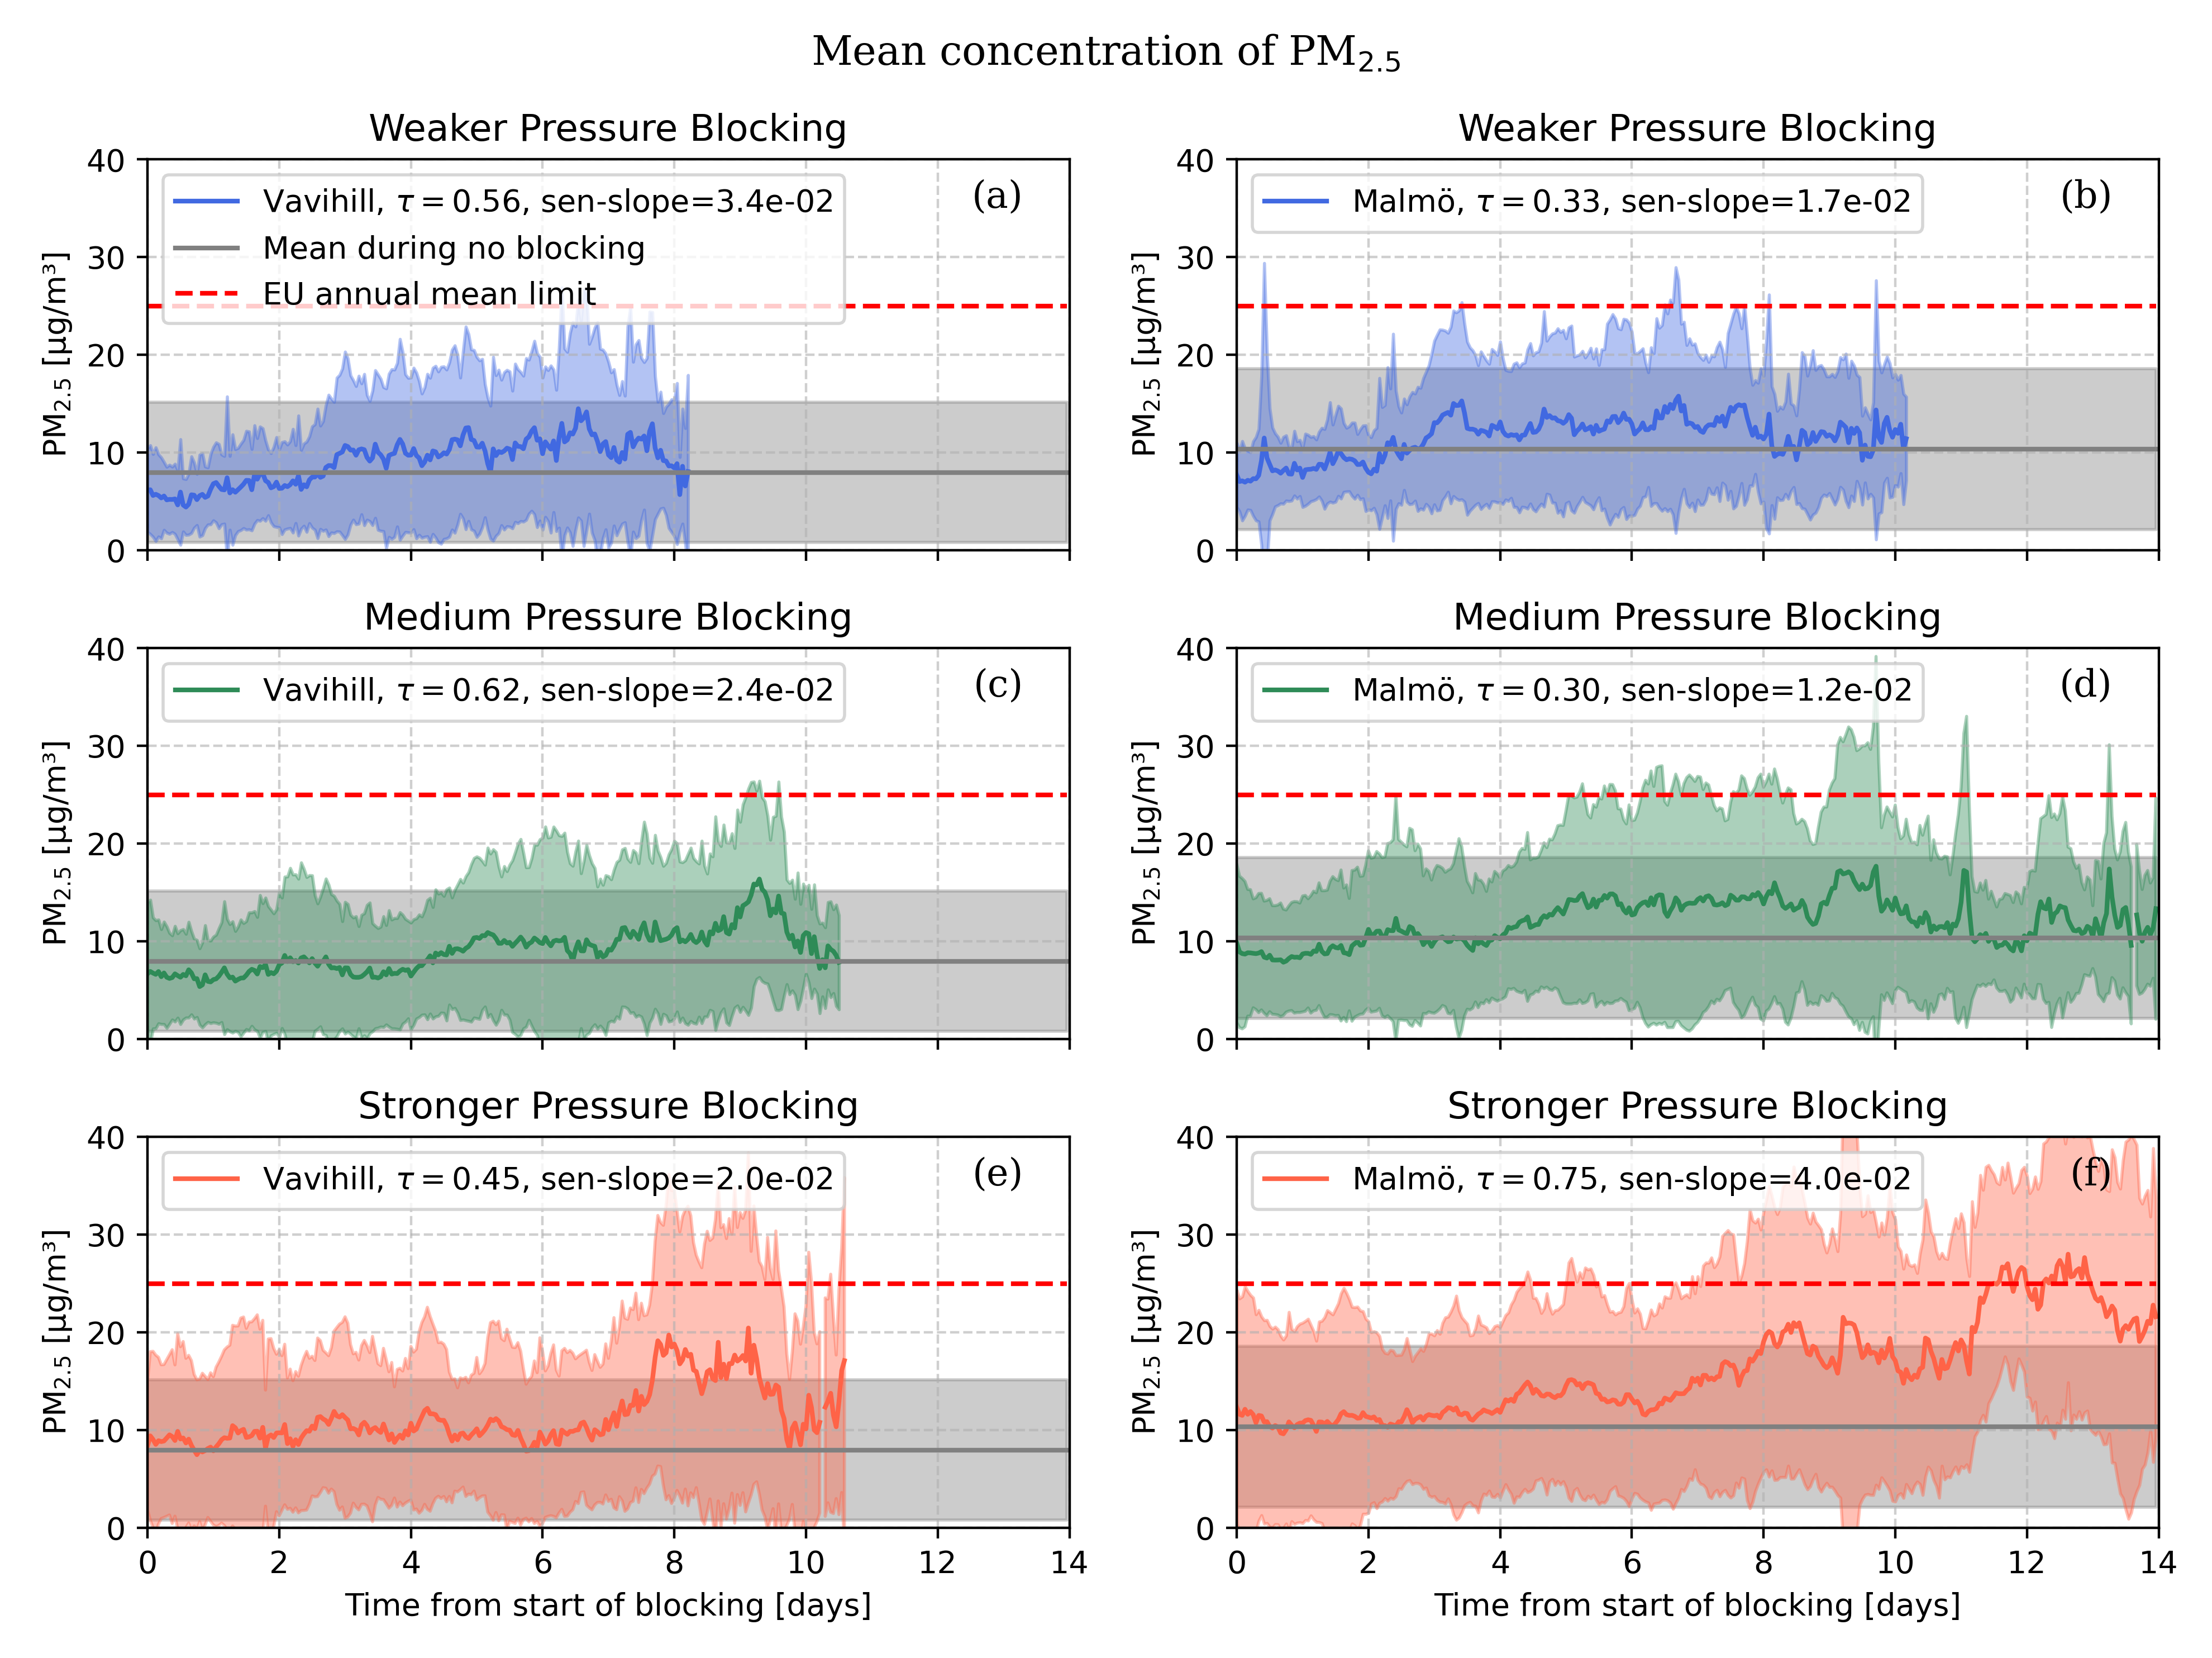
\includegraphics[width=\textwidth]{Figures/Meanplot_pressure.png}
        \caption{\PM concentrations in Vavihill and Malmö for different pressure strengths during high-pressure blocking events. This is shown by the blue line, the mean during no high-pressure blocking event can be seen by the grey line and the EU annual mean limit is displayed by the red line. The shaded regions indicates the standard deviation of the data.}
        \label{fig:Meanplot_pressure}
\end{figure}
 

Figure~\ref{fig:Meanplot_Comparison}--\ref{fig:Meanplot_pressure} all had a p-value, from the Mann-Kendall test, of their respectively increase approximately equal to 0, providing significant results. From Figure~\ref{fig:Meanplot_Comparison}--\ref{fig:Meanplot_pressure} it is clear that the high elevations of \PM occur after eight to thirteen days. These results indicates that prolonged periods of high-pressure blocking events indicate an accumulative increase of \PM, which can be seen in \autoref{fig:Meanplot_Comparison} where one can see that the combination of all the other plots resulted in a steady increase in the case of Malmö, and an increase in the case of Vavihill. The only case where no increase is observed is when the wind direction is from the northeast (see \autoref{fig:Meanplot_wind} a-b), which is not very common. This result indicates that for high-pressure blocking events one observes an increase in the concentration of \PM after eight to thirteen days regardless of the type of high-pressure blocking event, even though different types of high-pressure blocking events may differ in their specific increase. Especially strong increases with elevated \PM levels could be seen with winds from the southeast and for stronger high-pressure blocking events. 

\subsection{The Frequency of High-Pressure Blocking Events}
The last task was to determine whether high-pressure blocking events have become more common. When observing the number of high-pressure blocking events per year, no significant change in frequency could be seen (see \autoref{fig:number_of_blockings}). Since the highest levels of \PM  occurred toward the end of the events (see Figure~\ref{fig:Meanplot_Comparison}--\ref{fig:Meanplot_pressure}), the frequency of longer high-pressure blocking events was also examined. However, no increase could be observed in any of the cases. More interestingly, a small decrease can be observed from the $\tau$-values and the Sen's slope values. However, one must note that the p-values, from the Mann-Kendall test, are much larger here than Figure~\ref{fig:Meanplot_Comparison}--\ref{fig:Meanplot_pressure}. 

\begin{figure}[H]
    \centering
    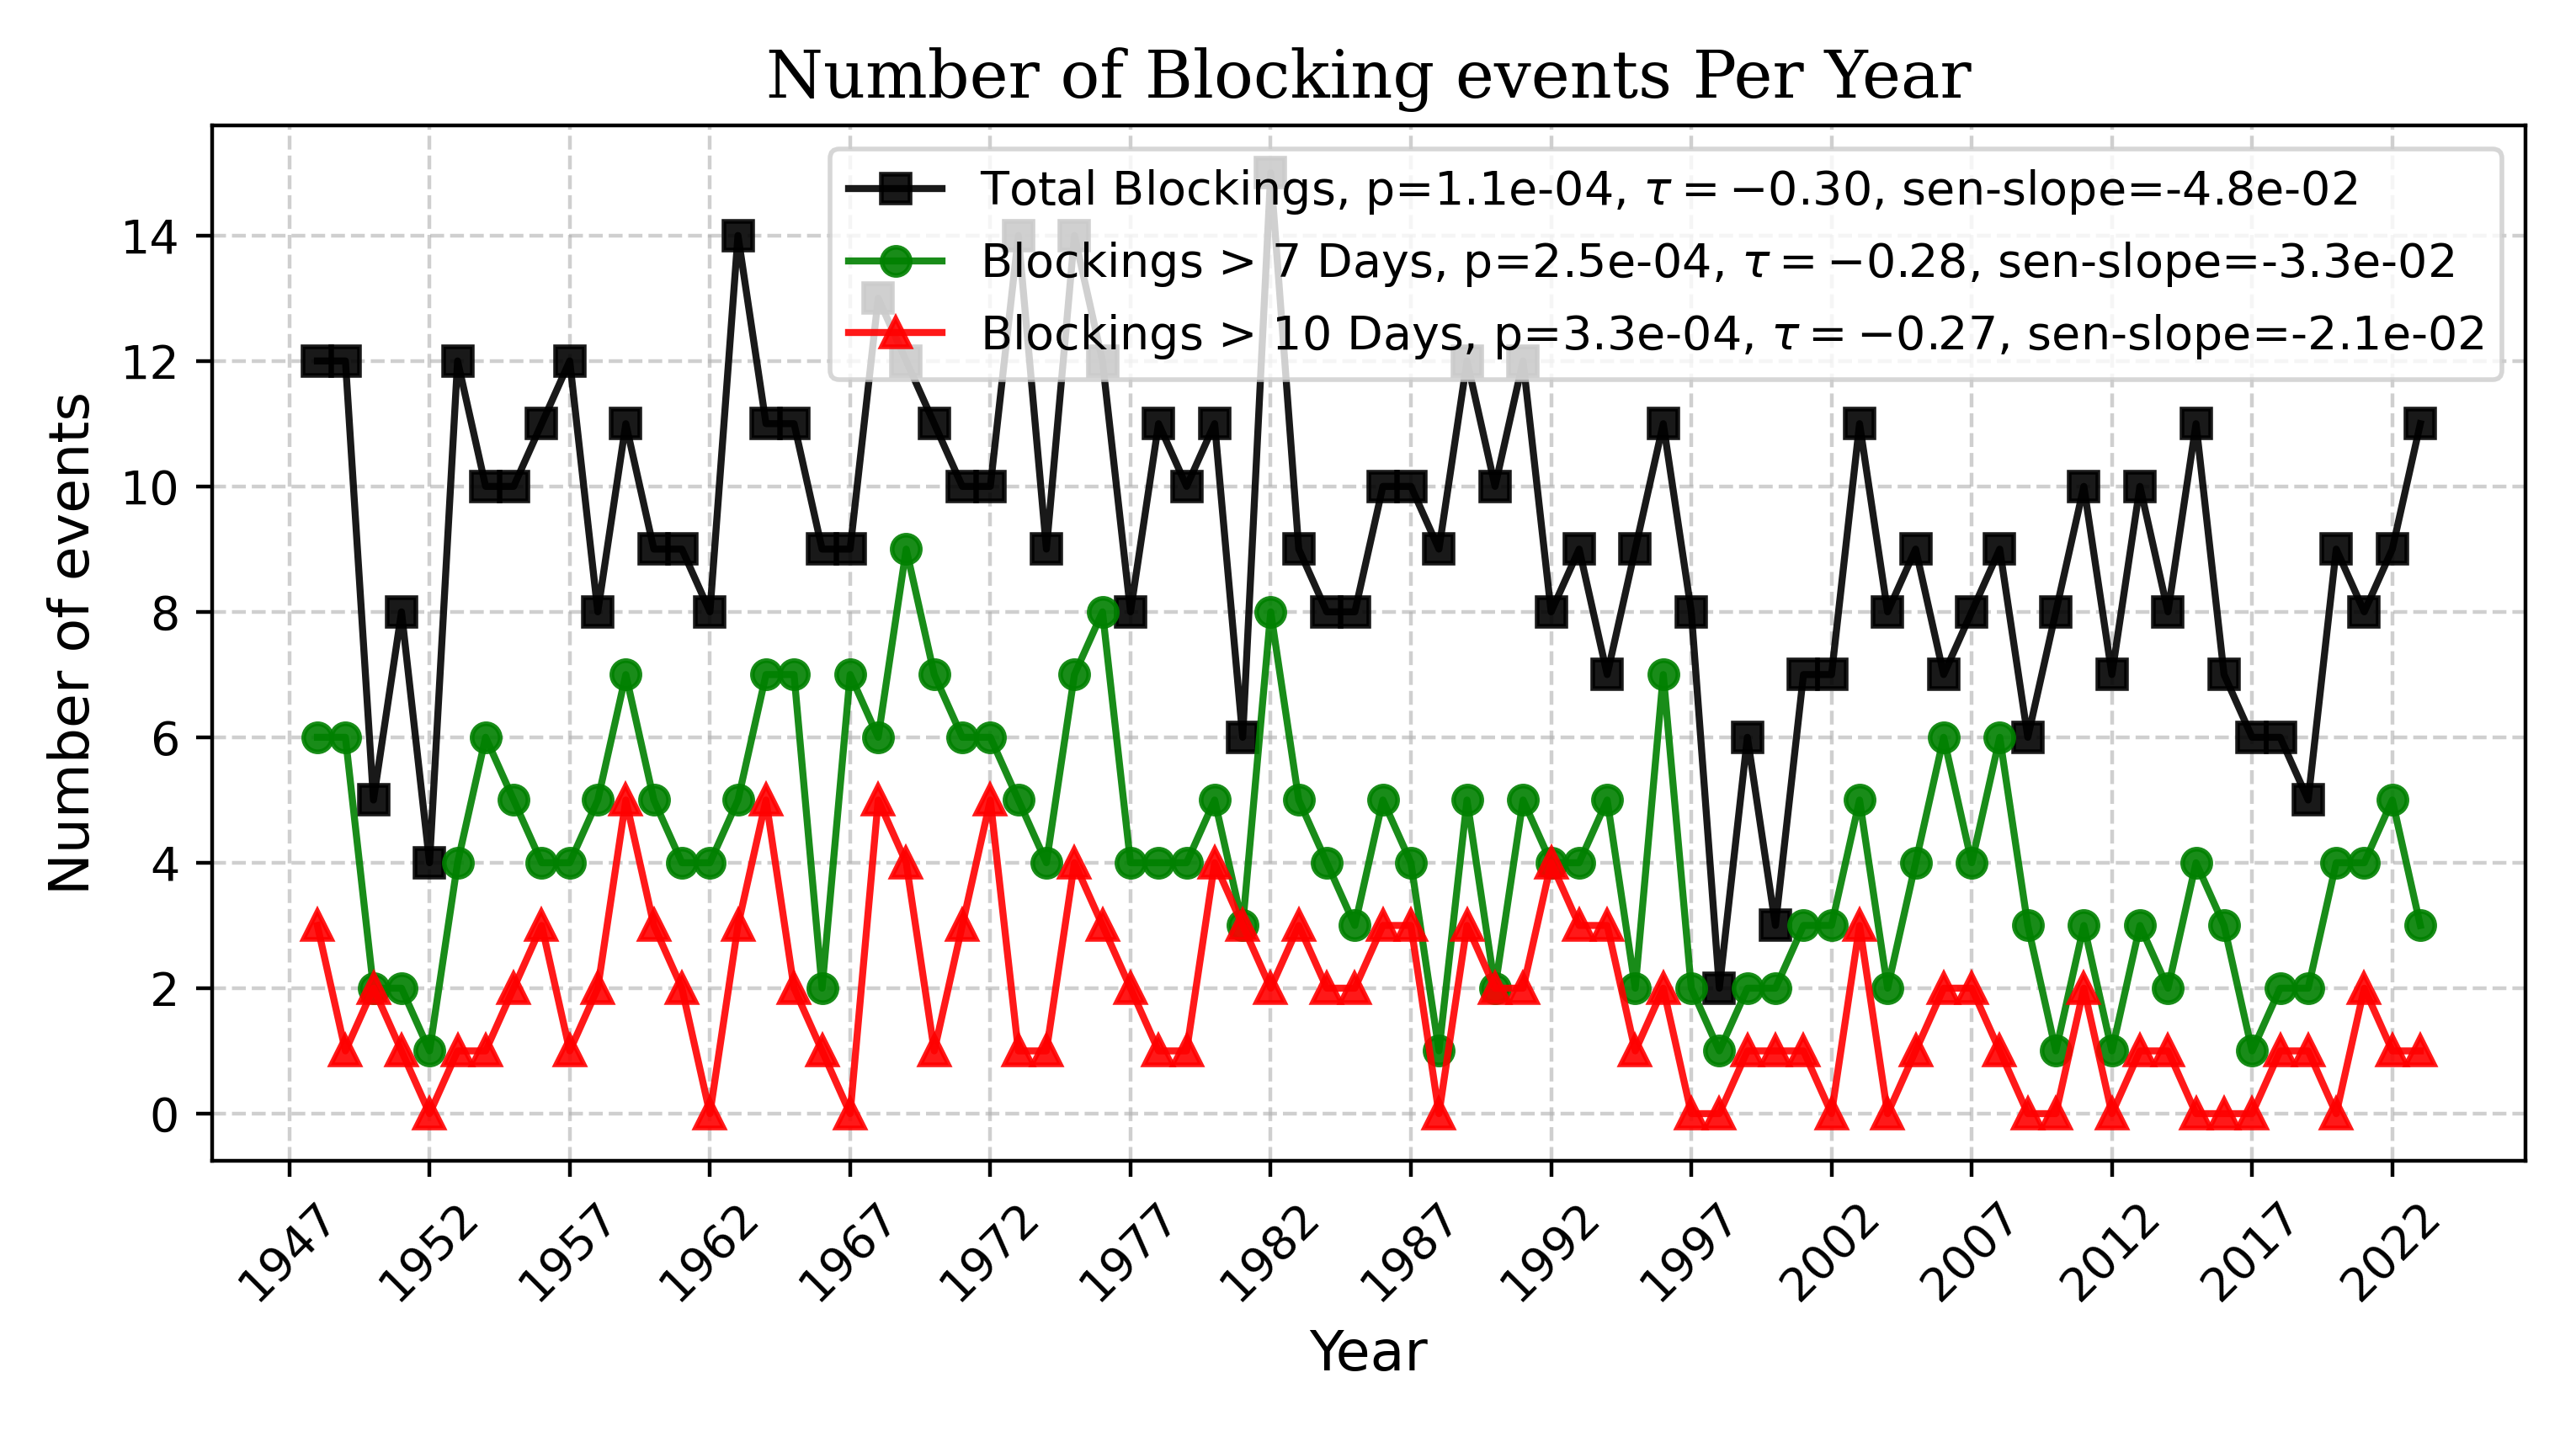
\includegraphics[width=0.7\textwidth]{Figures/BlockingsPerYear.png}
    \caption{fig: This plot show the change in frequency of high-pressure blocking events. The plots also indicates the change in events longer than seven and ten days. }
    \label{fig:number_of_blockings}
\end{figure}

In \autoref{fig:Number_of_Blocking_Days_Per_Year}, the number of days with high-pressure blocking events per year can be seen. Here, the total, seasonal, and pressure strength dependence can be observed. The reason for not including the directional dependence is that no wind data was available for this period. Even here a slight decrease can be seen in most plots, especially the total blocking days per year (h). 


\begin{figure}[H]
    \centering
    \includegraphics[width=\textwidth]{Figures/blocking_days_per_year_all.png}
    \caption{The number of days under a high-pressure blocking event each year, during each season, and for different pressure strengths. If the p-value was greater than 0.05, the corresponding $\tau$-value and Sen's slope were discarded, as the test was deemed statistically insignificant.} 
    \label{fig:Number_of_Blocking_Days_Per_Year}
\end{figure}

When observing the slight decline of the frequency of the high-pressure blocking events in \autoref{fig:number_of_blockings} and \autoref{fig:Number_of_Blocking_Days_Per_Year} one must note that the low $\abs{\tau}$-values indicate that the trend is not monotonic. Furthermore, the large p-values in \autoref{fig:Number_of_Blocking_Days_Per_Year} indicate that the trend is more random in comparison to the mean aerosol concentration plots observed in Figures~\ref{fig:Meanplot_Comparison}--\ref{fig:Meanplot_pressure}. One can observe that no type of high-pressure blocking events has become more common during the last 74 years. This is an interesting result since this aligns with the observations from other studies, where a decline of high-pressure blocking events has been observed during the late 20th century \cite{lupoAtmosphericBlockingEvents2020}. 
